% =====================================================================
%  Scientific Reports submission -- condensed "fast-read" version
%  Derived ONLY from the source manuscript (see CHANGELOG.md and
%  number_check.md).  No new data, numbers, claims, citations or figures.
%
%  Title candidates (both contain "validation-first"/"measurement
%  validity" and "resilience"; darknet/Bitcoin appear only as scenario
%  words, in the body, never in the title):
%    T1 (used):   Validation-first measurement of resilience in illicit
%                 data economies: a controlled study with a negative-result
%                 ledger on public data
%    T2 (alt):    Measuring resilience under measurement validity: a
%                 validation-first protocol and negative-result ledger for
%                 illicit data-trading ecosystems
%
%  Class note: the official Scientific Reports class (wlscirep.cls) was not
%  available offline, so a self-contained article-based layout with the same
%  single-column, wide-measure style is used.  It compiles with pdflatex and
%  the class can be swapped at submission without touching the content.
% =====================================================================
\documentclass[10pt,a4paper]{article}

\usepackage[utf8]{inputenc}
\usepackage[T1]{fontenc}
\usepackage{lmodern}
\usepackage[a4paper,margin=2.1cm]{geometry}
\usepackage{graphicx}
\usepackage{amsmath,amssymb}
\usepackage{booktabs}
\usepackage{array}
\usepackage{longtable}
\newcolumntype{L}[1]{>{\raggedright\arraybackslash}p{#1}}
\usepackage{textcomp}
\usepackage[numbers,sort&compress]{natbib}
\usepackage[hidelinks]{hyperref}

\setlength{\parskip}{2pt}
\setlength{\parindent}{12pt}
\renewcommand{\arraystretch}{1.12}

% Pack floats so they share pages with text instead of forcing float pages.
\renewcommand{\topfraction}{0.92}
\renewcommand{\bottomfraction}{0.75}
\renewcommand{\textfraction}{0.06}
\renewcommand{\floatpagefraction}{0.72}
\setcounter{topnumber}{3}
\setcounter{bottomnumber}{2}
\setcounter{totalnumber}{4}

\title{\bfseries Validation-first measurement of resilience in illicit data
economies: a controlled study with a negative-result ledger on public data}

% Author block carried over unchanged from the source submission (the real
% names, affiliation and funding are preserved verbatim; Scientific Reports
% is single-anonymous, so no anonymised variant is used).
\author{Ziying Xue\textsuperscript{1}, Yongjin Chen\textsuperscript{1},
Songze Zhu\textsuperscript{1,*}}
\date{}
\begin{document}

\maketitle
\thispagestyle{empty}

\noindent\textsuperscript{1}People's Public Security University of China,
Muxidi campus, 1 Muxidi Nanli, Xicheng District, Beijing 100038, China.\\
\noindent\textsuperscript{*}Corresponding author: 704339163@qq.com

\vspace{6pt}

\begin{abstract}
\noindent\textbf{Background.} Enforcement repeatedly disrupts illicit
data-trading ecosystems, yet whether they absorb a shock and resume function is
rarely measured under controls able to reject it.

\noindent\textbf{Methods.} We state a validation-first protocol: every quantity
must survive a control capable of falsifying it. We apply it to the social,
financial and infrastructure layers of an illicit data economy, from public
archives (the AlphaBay archive, the Elliptic++ Bitcoin graph, the Abuse.ch
URLhaus and ThreatFox feeds). Seven controlled analyses share one rule.

\noindent\textbf{Results.} Infrastructure is churn-dominant: median online
lifetime is \textbf{1.36} days, yet \textbf{13.88}\% of darkened hosts return
within one day against a \textbf{2.24}\% matched floor (\textbf{6.2}$\times$).
Displacement after the November 2019 Cryptonia--Cannazon shutdown is directional
(\textbf{+10.5} percentage points on Apollon; \textbf{+0.0} on Empire,
unmeasurable) but bounded, not estimated. The illicit financial subgraph is
peripheral: removing all \textbf{14,266} illicit-labelled addresses
(\textbf{1.734}\%) leaves the giant component at \textbf{98.88}\%.

\noindent\textbf{Conclusions.} Of six resilience metrics, none passes all three
validity gates. A negative-result ledger records that temporal-graph prediction
fails four independent instrument checks through a feature-side separability
trap, partially repaired by de-leakage.
\end{abstract}

\vspace{2pt}
\noindent\textbf{Keywords:} cybercrime ecosystems; network resilience;
measurement validity; darknet markets; temporal graph neural networks;
negative results.

\vspace{4pt}
\hrule
\vspace{6pt}

\section{Introduction}

Measuring how a system absorbs a shock and resumes function is hard wherever
three conditions hold at once: there is no ground truth, the observations are
censored, and the events are too few to estimate from. In such settings a
resilience number is only as trustworthy as the control it is run under, and a
control that cannot reject anything looks exactly like a control that rejected
nothing. We therefore treat that measurement problem --- how to construct a
falsifiable measurement of resilience in a system with no ground truth, censored
data and rare events --- as the primary object of study, and apply the resulting
protocol to one concrete domain.

Illicit data-trading ecosystems are one such system, and enforcement against
them is frequent and visible: in July 2017 Operation Bayonet seized AlphaBay and
secretly operated its successor Hansa, and the sites went down. The immediate
disruption was total, but what the surrounding ecosystem did next is far less
clear, because the archives are right-censored at a single instant, the layers do
not share a time axis, and no external ground truth certifies which actors are
illicit. We measure all three layers of this economy --- social, financial and
infrastructure --- from public data, and we report the null alongside the
estimate wherever a control was able to reject it.

Existing work reports quantities but rarely pairs them with controls shown to be
capable of rejecting the naive alternative. Longitudinal measurement established
the darknet-marketplace field and its displacement dynamics: the first
longitudinal measurement of the anonymous-marketplace ecosystem
\citep{soska2015measuring}, the collective recovery of dark-web marketplaces
after individual closures \citep{elbahrawy2020collective}, and vendor migration
from AlphaBay and Hansa into Dream Market after Bayonet
\citep{vanwegberg2018lost}. The same literature records the absence of any
durable reduction in cryptomarket activity after Operation Onymous
\citep{decaryhetu2017police}. It also documents the two
mechanisms a measurement has to disentangle: displacement into successor
platforms \citep{goonetilleke2023hydra}, and the reputation-transfer problem that
governs whether a vendor can move at all \citep{norbutas2020reputation}.

Graph learning supplies labelled illicit-transaction benchmarks and
node-classification baselines --- the Elliptic transaction graph and its GCN
baseline \citep{weber2019antimoney}, the address-level Elliptic++ with
heterogeneous-GNN baselines \citep{elmougy2023demystifying}, and purpose-built
anti-money-laundering datasets \citep{xiang2023babd,schnoering2025bitcoin}. Our
contribution is ecosystem measurement rather than classification, and our
negative result shows that even that transfer is unsafe without instrument
checks.

Network robustness theory explains why targeted removal beats random removal on
synthetic or reconstructed graphs \citep{albert2000error,ren2019generalized,duxbury2020responsiveness,cavallaro2020disrupting},
while evaluation-methodology work documents inflated baselines and leaky splits
\citep{shchur2018pitfalls,kapoor2023leakage,errica2019fair}. \emph{Negative
control} and \emph{pre-registration} are the classical names for the discipline
we adopt \citep{lipsitch2010negative,nosek2018preregistration}, and simulations
of criminal organisations under intervention remain rule-based rather than
data-driven \citep{manzi2024agentbased}.

\textbf{C1: a validation-first protocol.} Every candidate metric passes a
validity screen, every instrument is paired with controls required to be capable
of rejecting it, and every reported number carries the audit trail that lets a
reviewer reproduce the control applied to it. \textbf{C2: a controlled
measurement corpus.} Seven analyses span the social, financial and
infrastructure layers. Three claims survived their controls and four did not: a
headline ``3.7$\times$ more persistent'' claim was killed by an
immortal-time-bias control (\textbf{-0.49\,pp}), and a ``+3.64 reviews/week''
displacement estimate was demoted by its own non-centred placebo null to two
non-significant point estimates. The magnitude is therefore bounded rather than
estimated. \textbf{C3: a negative-result ledger.} Temporal-graph prediction of
recurrence fails four independent instrument checks, traced to a feature-side
separability trap that inflates shuffled-label controls, which de-leakage only
partially repairs; the hazard, its diagnosis and its partial repair are kept as
a result in their own right. The paper is organised as Data (\S2), Protocol
(\S3), Controlled analyses (\S4), Negative results (\S5), and Governance,
limitations and conclusion (\S6--\S7).

\section{Data}

The three layers share no time axis, and none of the datasets was collected for
the purpose of measuring resilience, so every cross-layer comparison in this
paper is an ordering rather than a ratio. All sources are public
(Table~\ref{tab:data}): the social layer is a full AlphaBay archive with Agora,
Kilos and drug-listing dumps, and the financial layer is the Elliptic++ Bitcoin
graph whose 49 ordinal steps anchor from outside the data to approximately
2016-01-01 to 2017-11-03. The infrastructure layer is the Abuse.ch URLhaus
and ThreatFox feeds, which are rolling-retention and current through
2026-09-23. Eight sources are public archives used under research terms, two are
Gwern-curated archives with no explicit licence used under research fair use,
and one context source is not used as evidence; no raw leaked personal records
are touched and identifiers are hashed.

\begin{table}[t]
\caption{Data sources. Sizes count parsed records in the processed archives.
The three layers share no time axis; per-source time coverage, and the Hansa and
Valhalla dumps (51,553 reviews and 16,511 listings, from which no reported
quantity is drawn), are detailed in Supplementary Note S5.\label{tab:data}}
\footnotesize
\setlength{\tabcolsep}{4pt}
\begin{tabular}{@{}p{1.6cm}p{3.6cm}p{5.6cm}p{4.4cm}@{}}
\toprule
\textbf{Layer} & \textbf{Source} & \textbf{Size} & \textbf{Licence}\\
\midrule
Social & AlphaBay full-site archive & 114,231 active listings; 1,217,388 feedback records & Gwern-curated; no explicit licence\\
Social & Agora market archive & 109,689 listings & Gwern-curated; no explicit licence\\
Social & Kilos cross-market review panels & 235,326 reviews & community mirror\\
Social & Drug-listing corpus & 194,433 listings & Gwern-curated; no explicit licence\\
Financial & Elliptic++ transactions & 203,769 nodes / 234,355 edges / 183 features & public dataset, research use\\
Financial & Elliptic++ addresses & 822,942 addresses / 2,868,964 address--address edges / 56 features & public dataset, research use\\
Infrastructure & Abuse.ch URLhaus & 58,310 takedown records & free for research, attribution requested\\
Infrastructure & Abuse.ch ThreatFox & 105,999 IOC records & free for research, attribution requested\\
External context & Monthly global breach-posture reports & 9 issues (2025-01 \ldots{} 2025-11, 05 and 09 absent) & context only; not used as evidence\\
\bottomrule
\end{tabular}
\setlength{\tabcolsep}{6pt}
\end{table}

\section{A Validation-First Measurement Protocol (C1)}

No quantity enters this paper until it has passed three gates, in order, and the
gates are stated in general terms rather than tailored to the one domain we
demonstrate them on (Fig.~\ref{fig1}).

\textbf{G1: metric validity.} A resilience metric must (a) recover a
ground-truth planted value in synthetic data, (b) distinguish real measurements
from randomised controls, and (c) respond to the construct it claims to measure.
Six candidate resilience metrics were screened against three pre-registered
criteria --- rank recovery against a planted truth \emph{without} collapsing onto
another metric's truth, calibration whose slope interval covers 1 and intercept
interval covers 0, and separation from a week-permuted null. \textbf{Each
criterion passes two of the six metrics, and no metric passes all three.} The
metric with the highest own-truth correlation (\texttt{recovery\_time}, Spearman
0.9859) fails the rank criterion precisely because it is indistinguishable from
\texttt{centrality\_redistribution} (max $|$cross-Spearman$|$ = 0.8407 $\geq$
0.8). The two metrics that pass the rank criterion fail the permutation
criterion by construction, since a time-invariant structural quantity cannot
separate from a week-permuted control.

\textbf{Reporting a failure is itself a result.} Because the artifact lists the
three criteria without stating a conjunction rule, any single count of survivors
is a post-hoc choice, so we report the per-criterion matrix rather than a score
(Supplementary Note S2). A metric that fails is either not reported or reported
together with its failure; the six metric \emph{names} come from the
pre-registered plan while their operational definitions are ours, so none of
this validates the delivered measure.

\textbf{G2: instrument validity.} An estimator or predictor must be paired with
controls that \emph{can} reject it: a negative-control band with a pre-registered
usable window \citep{lipsitch2010negative}, permutation tests, and a
shuffled-label control repaired against feature-side separability. Every design
is registered before it is run \citep{nosek2018preregistration}. A control whose
value is fixed by construction is not a control, because G2 requires
demonstrating that the control varies within the stratification the metric uses.
We found that failure three times: in two single-feature arms whose retained
feature is constant within every bin, and in a de-leakage configuration whose
retained feature set is the stratifying variable itself. A control in that state
fails G2 by definition rather than by a margin, and a design that reports it as a
pass has not tested anything.

\textbf{G3: auditability.} Every reported number maps to a hash-verified
artifact in a manifest, or is flagged as not yet in it, and cross-artifact
quantities must be reproduced independently by two pipelines before they are
used. The manifest's domain is the result artifacts this study produced and its
time point is its own build; the boundary rule is reproduced with the manifest so
that the count can be recomputed rather than taken on trust (Supplementary Note
S1). Two pipelines independently reproduced an address count of
\textbf{61,487}, the rare cross-artifact agreement that licenses a reading.

CPU and GPU replicates are never tabulated together: on one replicate the
largest per-cell absolute difference in reported AUC was max $|d|$ = 0.0068
against a pre-registered tolerance of 1e-3. Device-equivalence checks under fp64
deterministic mode reproduce bitwise across devices, whereas fp32 forward passes
exhibit chaos amplification and are excluded from equivalence gates. Discipline
of this kind is what makes a negative result interpretable, and what allows a
failed instrument to be reported as a diagnosis rather than as a gap.

\textbf{The two-list rule.} When an instrument self-reports failure, the failure
report itself is that gate's output and must be given: how many cells fell
outside the window, which cells they were, what the window was, and the verbatim
decision rule. What is forbidden is any quantity \emph{read off} the failed
instrument --- a point estimate, a band, a comparison, a significance statement.
The test for which list a reading belongs to is whether it can stand without the
failed instrument: cell identities and the window cannot and are therefore
reportable, whereas a shuffled-control AUC can and is therefore withheld.

\textbf{The feature-side separability trap.} G2 is where existing practice is
thinnest, because a control that cannot reject anything looks exactly like a
control that rejected nothing. In censored ecological graphs, labels are
frequently derived from the same structural statistics that are also features ---
degree, transaction counts, address statistics --- so shuffling the labels does
not break the feature--label association and a shuffled-label control reads far
above chance. The instrument that did not fail here is the permutation null: it
uses \textbf{4000 draws}, one band per pre-registered horizon, and permutes time
steps rather than nodes. On our data the shuffled-label control reads
\textbf{0.71364} at $\Delta = 1$ against a permutation band of
\textbf{[0.4852, 0.5148]}, and the instrument's verdict is OUTSIDE.

\textbf{What anchors 0.5.} A control whose score is independent of the label
\emph{by construction}, read through the same within-entry-step weighted
estimator the arms are judged on, reads 0.4897--0.5141 (largest absolute
deviation 0.01406). So on this data \textbf{0.5} is the right anchor and the
shuffled control's distance from it is real. What that distance does \emph{not}
license is calling it leakage, because the excess conflates feature-side
separability with label leakage, is not decomposable, and is therefore not
published as any number.

\textbf{How far the repair goes.} Readings are within-entry-step weighted at
$\Delta = 1$. Dropping the calendar column reads 0.71556 and dropping the
position column reads 0.71758 --- both \emph{higher} than the as-built
\textbf{0.71364}, so removing either column repairs nothing. The attribution is
carried by the two arms that move the reading by more: the six family-mean
features alone read 0.69372 and the two family-count features alone read 0.56115.

Retraining on reduced feature families does not return the control to chance:
the strongest non-vacuous configuration moves the reading from \textbf{0.71364}
to \textbf{0.6561} and stops there (configuration-by-configuration accounting in
Supplementary Note S3). Two arms read exactly 0.5, but that is a construction
artefact: a single feature constant within every bin yields an AUC of exactly
one half, so those are vacuous controls rather than evidence of cleanliness. The
transferable lesson is that in this measurement domain a shuffled-label control
is not automatically a null model, and the first thing to check is whether it can
vary at all.

\begin{figure}[htbp]
\centering
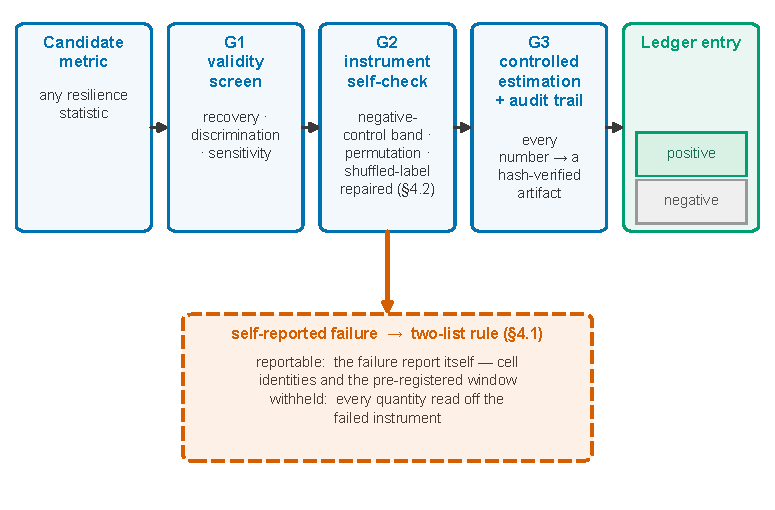
\includegraphics[width=0.78\textwidth]{figures/02_protocol_flow.pdf}
\caption{The five-step protocol. A candidate metric enters the G1 validity
screen and, if it survives, the G2 instrument self-check, then controlled
estimation with its audit trail (G3), ending in a ledger entry that records a
positive or a negative result. The red side branch is the protocol's most
distinctive move: when an instrument self-reports failure at G2, the failure
report itself becomes that gate's output under the two-list rule, while every
quantity read off the failed instrument is withheld.\label{fig1}}
\end{figure}

\section{Controlled Analyses (C2)}

Each of the seven analyses follows the same four-part structure --- the
question, the design, the control that bites, and the finding with its bound ---
and in four of the seven the control that bites took down a claim of our own.
One caveat belongs before the first of them: the seven are not seven independent
studies. The displacement analysis in \S\ref{sec:e1v3} and the exploratory
cross-layer association (Supplementary Note S2) share a panel, an estimator and
the same November 2019 event, so the latter is in substance an audit of the
former that found the pre-trend the earlier design had missed. The number of
independent events behind this corpus is therefore smaller than seven.
Table~\ref{tab:analyses} gives the whole corpus at a glance; full controls and
every rejected estimator are in Supplementary Note S2.

\begin{table}[t]
\caption{The seven controlled analyses: the quantity that survived each one, the
layer it belongs to, the control that bit, and what that control rejected. Four
of the seven controls took down a claim of our own.\label{tab:analyses}}
\scriptsize
\setlength{\tabcolsep}{3pt}
\begin{tabular}{@{}L{1.75cm}L{1.55cm}L{4.35cm}L{3.35cm}L{5.0cm}@{}}
\toprule
\textbf{Analysis} & \textbf{Layer} & \textbf{Headline quantity} & \textbf{The control that bites} & \textbf{What it rejected}\\
\midrule
\textbf{E7-inf} Host reconstitution after takedown & Infrastructure & \textbf{13.88\%} of hosts return within 1 d vs a \textbf{2.24\%} matched chance floor (\textbf{6.2$\times$}) & Within-host paired design (removes immortal-time bias) & The naive \textbf{3.7$\times$} advantage; controlled, \textbf{-0.49 pp} with the sign reversed (p = 8.1e-07)\\
\textbf{E0} Survival after listing & Infrastructure & Median online lifetime \textbf{1.36 days}; S(1 d) = \textbf{0.6064}, S(7 d) = \textbf{0.1575}, S(30 d) = \textbf{0.0497} & Site- and reporter-clustered SEs & Concentration proposition: \textbf{p = 0.1736} by reporter, \textbf{p = 0.5978} by block, both non-significant; IID understated the SE by \textbf{14.44$\times$}\\
\textbf{E4} Product survival in the social layer & Social & Median \textbf{222.9 days} overall vs \textbf{10.8 days} reviewed; the gap \emph{is} the censoring & Proportional-hazards test; outcome definition & The model read as a transaction process: the outcome is first recorded feedback, and proportional hazards is violated for \textbf{19 of 24} covariates\\
\textbf{E1-v3} Directional displacement after a market seizure & Social & Exposed vendors appear on Apollon \textbf{+10.5 pp} above matched controls; the Empire cell is \textbf{+0.0 pp}, a zero denominator & Non-centred placebo null (500 draws) & The intensive-margin estimate \textbf{``+3.64 reviews/week''}; its own null is centred at \textbf{+1.1156}, a parallel-trends violation, so it is demoted; corrected magnitude \textbf{+1.0 to +2.4}\\
\textbf{E5-fin} Financial-layer recurrence & Financial & Recurrence \textbf{7.4716\%} (n = 61,487), graded across label classes & Specificity test across two enforcement-indistinct classes & The causal reading of the gradient: the licit--unknown gap (\textbf{-2.470 pp}) nearly equals the illicit--licit gap (\textbf{-2.735 pp})\\
\textbf{E6-fin v2} Structural position of the illicit subgraph & Financial & Random removal must delete \textbf{60.0\%} of nodes to halve the giant component; degree-targeted removal does it at \textbf{2.5\%} & Saturation check; pre-specified window test & The dismantling reading: saturated at \textbf{47 of 49} steps (sd = 0.000043), so the metric cannot register a shock; the pre-specified July 2017 window does not reject (\textbf{p = 0.0954}, \textbf{0.3458})\\
\textbf{E3} Causal attribution of resilience & Social $\leftrightarrow$ Financial & No matched design reaches cluster-robust p \textless{} 0.05; the licensable result is an absence (H4: \textbf{$\beta$ = -0.5804, p = 0.8047}) & Propensity-score overlap; direct measurement of the H2 substrate & The PSM design (\textbf{overlap = 0.000}, zero pairs, max $|b|$ = \textbf{20.61}) and the H2 bridging mechanism: \textbf{124} valid BTC addresses, \textbf{three} in Elliptic, all non-transactional\\
\bottomrule
\end{tabular}
\setlength{\tabcolsep}{6pt}
\end{table}

\subsection{Host reconstitution after infrastructure takedown (E7-inf)}\label{sec:e7inf}

\textbf{Question.} After an IOC is taken down, how quickly does the hosting
infrastructure behind it reappear?

\textbf{Design.} Abuse.ch takedown records; hosts and domains tracked across
takedown events; reconstitution latency measured with stratified matched floors
for chance re-appearance and within-host pairing for infrastructure reuse.

\textbf{The control that bites.} A naive comparison suggested that reusing
infrastructure confers 3.7$\times$ more persistence. A within-host paired design,
which removes the immortal-time bias that creates the illusion, reverses the
sign to \textbf{-0.49 percentage points} (sign test p = 8.1e-07), and the small
negative effect strengthens as bulk hosts are dropped. The naive number is a
bias exhibit, not a finding.

\textbf{Finding.} Median takedown delay spans \textbf{0.47--1.52 days} across
treatments that bracket the unobserved times. Fully darkened hosts do come back:
\textbf{13.88\%} return within one day, \textbf{6.2$\times$} the stratified
matched chance floor of \textbf{2.24\%}, and about 21\% within a week.
Domain-hosted infrastructure returns more often than bare-IP infrastructure at
equal host size (\textbf{80.77\% vs 61.49\%} at more than 20 URLs, a factor of
1.31, against a paired control significant at p \textless{} 0.001). One control
here is vacuous by construction, and we report it as that rather than as a pass:
hosts carrying a single URL \emph{cannot} produce a later addition, and both
kinds read exactly 0.00\% against approximately 8\% floors (Fig.~\ref{fig2}).

\textbf{Bound.} These are reconstitution dynamics of observable infrastructure;
covert migration off these hosts is not measurable from takedown records, and
the feed carries an unknown admixture of scanner traffic. The result also
survives a change of aggregation scale: the week-7 reconstitution rate is not an
artefact of one window. Recomputed month by month across the \textbf{4} months
that clear the 100-record floor, the spread between the highest and lowest
monthly value is \textbf{7.667 percentage points}, against a 10,000-draw
permutation null spanning \textbf{[0.3612, 2.9833]} (p \textless{} 1e-4).

\subsection{Infrastructure survival after listing (E0)}

\textbf{Question.} How long does malicious infrastructure survive once listed?

\textbf{Design.} 36,262 queued URLhaus records inside the retention window;
event rate 93.2\%; Kaplan--Meier survival after first appearance.

\textbf{The control that bites.} A headline hypothesis, that concentration
(block-level hosting density) predicts longer survival, fails under clustered
standard errors (\textbf{p = 0.1736} clustered by reporter, \textbf{p = 0.5978}
clustered by infrastructure block) after the IID standard error turned out to
understate the block-clustered one by \textbf{14.44$\times$}. We report the
null, not the story. A second apparent effect, significant survival differences
across groups, reduces to a label-semantics difference between untagged
placeholder and source-probe groups, and is disclosed as such.

\textbf{Finding.} Median online lifetime is \textbf{1.36 days}; S(1 d) = 0.6064,
S(7 d) = 0.1575, S(30 d) = 0.0497, so half of listed URLs are gone within a day
and a half while about 5\% survive beyond a month. At the malware-family level
the pattern is robust: Mozi-tagged URLs are taken down about 1.6$\times$ as fast
as the rest (median 1.13 vs 1.81 days). Every duration here is a lower bound,
because \texttt{last\_online} records the last sighting of a URL rather than the
instant it was taken down. Short median lifetimes therefore coexist with the fast
reconstitution of \S\ref{sec:e7inf}: churn, not death, is the dominant
infrastructure dynamic. The curve is also stable over the observation window:
at the 14-day horizon the fitted logistic trend across cohort weeks is an odds
ratio of 1.0016 per day (interval [0.9999, 1.0034], p = 0.070), that is, no
trend.

\subsection{Product survival in the social layer (E4)}\label{sec:e4}

\textbf{Question.} How long do listings survive on a major market?

\textbf{Design.} AlphaBay archive, n = 114,231 listings, event rate 45.9\%;
Kaplan--Meier and Cox survival with covariates.

\textbf{The controls that bite.} The outcome is first recorded feedback, not
first transaction, so a listing that transacts without leaving feedback is
censored rather than counted, and the 45.9\% event rate is a lower bound on the
transaction rate. The two medians must therefore be reported together,
\textbf{222.9 days} overall versus \textbf{10.8 days} for the reviewed subset,
because the gap \emph{is} the censoring and quoting either alone misstates the
result. Proportional hazards is violated for \textbf{19 of 24} covariates and no
seller key exists, so we report Kaplan--Meier medians as descriptive and treat
every Cox coefficient as exploratory.

\textbf{Finding.} Listing-level persistence in the social layer is long relative
to infrastructure: median \textbf{222.9 days} against \textbf{1.36 days}, a
ratio of about 164. The two layers are not on a shared clock, so this is an
ordering of two different quantities, not a like-for-like duration ratio, and we
use it only to say which layer is the slower one.

\textbf{Bound.} No seller-level clustering is possible, so these are descriptive
quantities rather than effects, and the two social-layer panels that carry no
date column (Kilos, drug-listing) cannot contribute to the comparison at all.

\subsection{Directional displacement after a market seizure (E1-v3)}\label{sec:e1v3}

\textbf{Question.} After the November 2019 shutdown of Cryptonia and Cannazon,
where did exposed vendors actually go?

\textbf{Design.} Exposure-matched comparison of vendor appearance rates on
candidate successor markets; the final of three generations of this analysis,
the two earlier designs having been declined by their own falsification tests.

\textbf{The controls that bite.} Two, and both cut. The aggregate picture
(Apollon rising from 6.2\% to 68.4\% of ecosystem volume while Cryptonia and
Cannazon go to zero) is exactly what a collector re-weighting its coverage would
produce with nobody moving, so we report it as a description and never as an
effect.

And the original intensive-margin estimate of ``\textbf{+3.64 reviews/week}''
was killed by its own placebo machinery: the 500-draw placebo null was itself
centred at \textbf{+1.1156} (sd 0.3205), which \emph{is} a parallel-trends
violation, and the three placebos originally reported were all drawn below that
null's mean. The largest of three draws is therefore a selection minimum rather
than a characterisation of the null. The corrected magnitude, on the designs
whose nulls sit near zero, is \textbf{+1.0 to +2.4 reviews/week} against a
treated pre-period base of 1.15. One cell in the per-source breakdown
has a zero denominator (\textbf{Empire: 0.0\% against 0.0\%}, odds ratio
undefined) and is unmeasurable rather than a ``no effect''; a second
(\textbf{Cannazon}) rests on 10 events and is underpowered rather than confident.

\textbf{Specification choice.} We ask how much of the demoted estimate survives
the choices a reasonable analyst would make. Twelve core specifications ---
varying the fixed-effect structure, the binning, the event definition, the
target market and the pre/post window --- are all estimable, and every one is
positive and clears zero at the 5\% level. The curve is anchored to the
incumbent analysis rather than standing free, reproducing its coefficient
exactly when the candidate set is held equal. The coefficients themselves are
listed in Supplementary Note S2. What the curve is \emph{not} is a
rehabilitation of the magnitude: it varies the specification, not the placebo
machinery, so it does not re-test the parallel-trends violation that demoted the
estimate, and its breadth must not be read as an interval estimate.

\textbf{Finding.} Displacement is real and directional. Exposed vendors appear
on Apollon \textbf{+10.5 percentage points} above matched controls, and on the
shrinking market Empire \textbf{+0.0 points}, a zero-denominator cell that is
unmeasurable rather than a measured null. From the Cryptonia-exposed population
the odds ratio is \textbf{3.34 (p = 3.5e-6)}, against 0.968 for
Cannazon-exposed. Two markets died on the same day; one population substituted,
the other did not move.

\textbf{Bound.} Two bounds, neither decorative. The corrected figures are
\textbf{two non-significant point estimates} (+1.0424 at cluster-robust p = 0.36
and +2.4426 at p = 0.24), so we report \textbf{no interval estimate}. What the
placebo draws support is the existence of an effect, since the real coefficient
sits in the 96.8th--100th percentile of its own null; what they forbid is any
statement that the effect lies in a narrow band. And because treatment is
defined as activity on a target market \emph{and} on a market that died, part of
the +10.5 points is the same sellers' activity re-registering rather than
market-level substitution. So \textbf{+10.5\,pp is an upper bound on
substitution}; the qualitative point, that displacement has addresses and not
merely volume, is the robust content.

\subsection{Financial-layer recurrence (E5-fin)}

\textbf{Question.} After a node is flagged illicit in Elliptic++, how often does
activity recur through it?

\textbf{Design.} Recurrence of participation over the 49-step ordinal axis, by
label class, estimated within entry step so that the differing amount of room
available to late entrants is removed exactly rather than modelled.

\textbf{The control that bites.} The headline gradient (illicit \textbf{1.816\%}
\textless{} licit \textbf{5.796\%} \textless{} unknown \textbf{8.371\%};
\textbf{7.4716\%} overall) is not licensable as a class effect. A specificity
check comparing two classes that enforcement does not distinguish shows the
licit--unknown gap (\textbf{-2.470 pp}) nearly equals the illicit--licit gap
(\textbf{-2.735 pp}). A monotone gradient across all three labelling categories
is therefore as consistent with how addresses entered the labelled subgraph as
with anything about illicit behaviour. We report the gradient, withhold the
causal reading, and withhold every p-value, because between-step differences
span $-27.4$ pp to $+13.1$ pp, roughly 100$\times$ the nominal standard error, so
the fixed-effect standard error assumes a homogeneity the data plainly violates.

\textbf{Finding.} Recurrence exists at \textbf{7.4716\%} overall and is strongly
graded. This quantity anchors here because two independent pipelines reproduced
the classifying set at \textbf{61,487} identically, the rare cross-artifact
agreement that G3 demands.

\textbf{Bound.} The labels are dataset-internal and cannot be certified against
external ground truth, and the outcome is recurrence in the \emph{labelled}
subgraph rather than in Bitcoin, so an address ``dies'' here when it stops
touching that subgraph.

\subsection{Structural position of the illicit subgraph (E6-fin v2)}\label{sec:e6fin}

\textbf{Question.} What would network-level disruption of the financial layer
actually require?

\textbf{Design.} Dismantling analysis on the Elliptic++ address graph as one
aggregate snapshot (822,942 nodes), not on the 49 per-step snapshots: random
versus degree-targeted node removal, and full removal of the illicit-labelled
set. Two pre-specified tests accompany it.

\textbf{The controls that bite.} The giant-component metric itself nearly fails:
at \textbf{47 of 49} time steps connectivity is saturated at 1.0000 (sd =
0.000043), so per-step giant-component size cannot register a shock at this
resolution and the metric is usable only in the rare unsaturated steps.
Separately, a pre-specified test of the July 2017 enforcement wave does not
reject on any observable. The window was fixed at steps 41--43 before the run,
the direction as ``lower'', and the null drawn from 20,000 random 3-step
windows; the p-values are \textbf{0.0954} for illicit share and \textbf{0.3458}
for illicit address count, with a third observable moving the \emph{wrong} way.
We report this as a low-power test, not as evidence of absence.

\textbf{Finding.} Random removal must delete about \textbf{60\%} of nodes to
halve the giant component; degree-targeted removal does it at \textbf{2.5\%}
(Fig.~\ref{fig3}).
The asymmetry is between the two \emph{removal fractions} ($60/2.5 \approx 24$),
not between two effect sizes, and it carries the scale-free signature. Deleting
\textbf{all} illicit-labelled nodes (\textbf{14,266} nodes, \textbf{1.734\%} of
addresses) leaves the giant component at \textbf{98.88\%}, indistinguishable
from removing the same number at random, and targeting the illicit subgraph's
best-connected members does no better. The mechanism is visible in the degree
table rather than inferred: mean degree \textbf{3.645} for the illicit class
against \textbf{10.803} for the \emph{licit} class, so the contrast is illicit
against licit and not illicit against the whole graph.

\textbf{Finding, continued: where the illicit class sits.} The removal result is
one reading of the illicit subgraph's position, and the nested-core profile
agrees with it. The aggregate graph has degeneracy \textbf{768}, and the illicit
class sits nearer the outside of that nesting than the licit class: mean coreness
is 2.2114 for illicit addresses against 6.0496 for licit ones, a difference of
-3.8382 against a 10,000-draw permutation null spanning [-0.1825, 0.1912] (p
\textless{} 1e-4). The label is at the same time strongly assortative --- label
assortativity 0.7606 against a null spanning [-0.0027, 0.0019] --- so the two
readings are not in tension: the illicit label is very nearly a community of its
own, and that community is peripheral in the nested-core sense rather than
central.

Ranking four removal strategies by the area under the curve of cleared illicit
share against node budget gives \textbf{34.2723} for random, \textbf{19.9398} for
k-core-targeted, \textbf{5.2254} for degree-targeted and \textbf{1.4031} for
PageRank-targeted, every comparison against random significant at the permutation
floor over 16 seed pairs (p \textless{} 1e-4). Budget spent by coreness is
therefore spent on the licit core rather than on the illicit periphery. The
marginal-cost field, the node budget needed to clear 1\% of the illicit set,
reads 8229.4 for random, degree and PageRank alike and 65835.4 for k-core. That
field is right-censored by its own grid --- it takes the first grid point at
which the threshold is met --- so the ordering of strategies is carried by the
AUC readings, not by this field.

\textbf{Bound.} Address-level enforcement against illicit finance has no
network-level effect \emph{in this graph}, and this is the labelled subgraph,
whose composition is a collection artefact.

\subsection{Causal attribution of resilience (E3)}

\textbf{Question.} Which structural features cause faster recovery?

\textbf{Design.} Pre-registered hypotheses H1--H4 (decentralisation, cross-layer
bridging, functional redundancy, centrality), tested by propensity-score
matching plus difference-in-differences around the November 2019 shutdown, with
500 placebo event dates per design.

\textbf{The control that bites.} This analysis mostly did not survive. The
pre-registered PSM covariate set is infeasible because it contains
\texttt{n\_markets}, which treatment \emph{defines}, so treatment becomes
perfectly predictable and matching returns \textbf{overlap = 0.000} with zero
pairs (max $|b|$ = 20.61) --- a specification failure, not a vanishing effect.

Three reduced specifications match (121, 77 and 74 pairs) with point estimates
\textbf{+1.04, +1.42 and +2.44} reviews/week, and the second column of each
design gives +1.34, +3.64 and +4.49, for a range of +1.04 to +4.49. But the two
largest second-column values stand on placebo nulls whose means are not centred
at zero (\textbf{+0.6672} and \textbf{+0.6606} against a treated pre-period base
of 1.15), which is the condition \S\ref{sec:e1v3} uses to demote an estimate. On
the column whose three nulls sit near zero, the usable range is \textbf{+1.04 to
+2.44}. No matched design reaches cluster-robust p \textless{} 0.05, and the two
uncertainty measures disagree on the same design (cluster-robust p = 0.36,
placebo rank p = 0.022), so we report the divergence rather than choosing the
smaller number.

H3 has no class column and is unmeasurable, and the substrate for H2 was measured
and found not to exist: only \textbf{124} checksum-valid BTC addresses exist in
the entire social layer, \textbf{three} intersect Elliptic, and all three are
adjudicated non-transactional.

\textbf{Finding.} Of four hypothesised mechanisms, one returns a licensable
result, and what it licenses is an absence rather than a positive relation:
H4's centrality term is null (\textbf{$\beta$ = -0.5804, p = 0.8047}), while
H1's decentralisation term is positive but likewise non-significant
(\textbf{+2.4823, p = 0.2416}). The asymmetry is the point: H1 predicted a
positive interaction and H4 predicted no such relation, so the same
non-significance fails one and supports the other. Matching being infeasible,
the design falls back on 500 placebo draws per design, and every matched design
places its real coefficient in the 96.8th--100th percentile of its own null,
which supports ``an effect exists'' and forbids ``the magnitude is
such-and-such''. We report the design's failure as a bound on what this data can
ever say about mechanisms --- with a single ecosystem-wide shock, effect
magnitudes are not identified by any matching or placebo machinery.

\subsection{Cross-analysis synthesis}

Three findings survived their controls. (i) Churn dominates death at the
infrastructure layer (1.36-day medians, 6.2$\times$ reconstitution) while the
social layer persists (222.9-day medians), so resilience sits in the fast layer
and persistence in the slow one. (ii) Displacement is directional: it has
addresses, but the corrected figures are two non-significant point estimates
(+1.04 and +2.44 reviews/week), not an interval. (iii) The illicit financial
subgraph is a periphery, not a core, which bounds what address-level enforcement
can achieve. These are not the same quantity measured twice: different
populations, different censoring mechanisms and different event definitions, on
layers that share no time axis.

\begin{figure}[htbp]
\centering
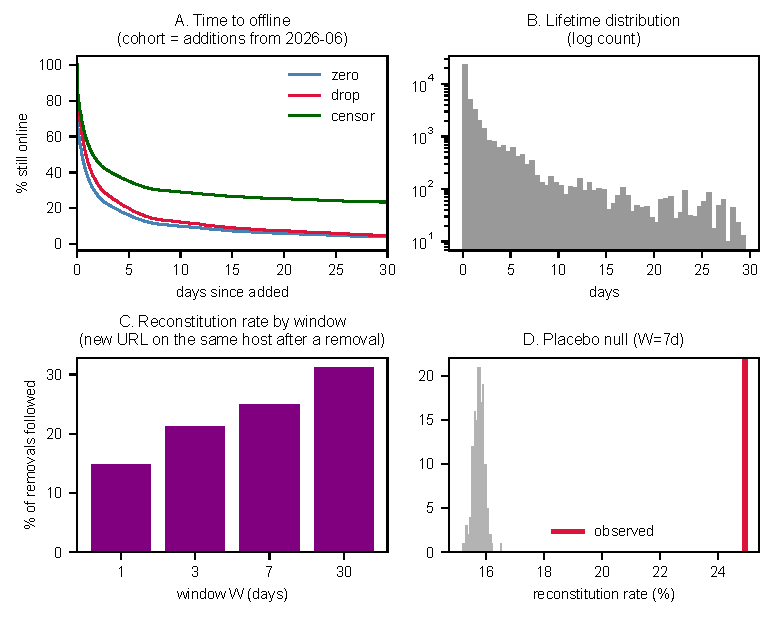
\includegraphics[width=0.58\textwidth]{figures/E7inf_v2.pdf}
\caption{Reconstitution of hosting infrastructure after takedown (E7-inf), in
four views. (a) Time from first sighting to going offline, for the cohort added
from 2026-06. (b) The same lifetimes on a logarithmic count axis.
(c) Reconstitution rate against the observation window. (d) Placebo null at
$W = 7$ days, so the observed rate is read against its null and not against
zero. Every duration is a lower bound.\label{fig2}}
\end{figure}

\begin{figure}[htbp]
\centering
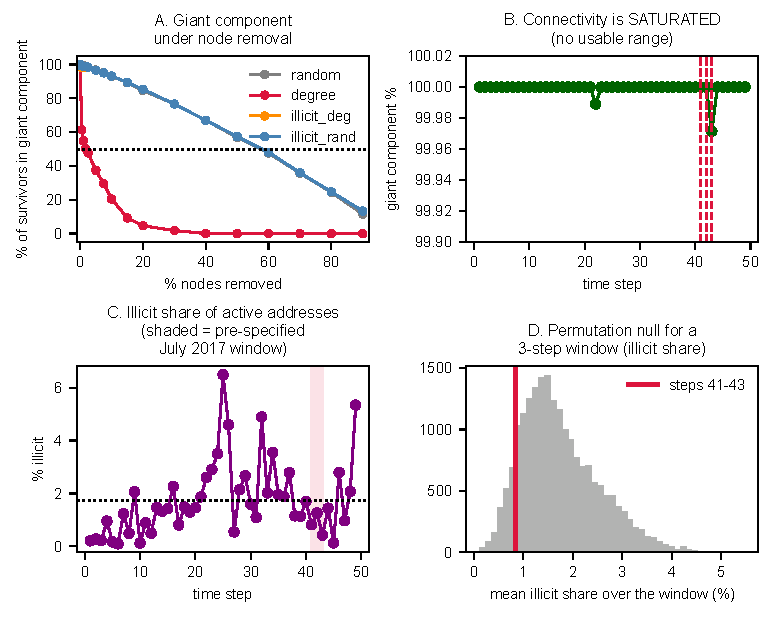
\includegraphics[width=0.58\textwidth]{figures/E6fin_resilience_v2.pdf}
\caption{Dismantling the illicit subgraph (E6-fin), four views on the
Elliptic++ address graph as one aggregate snapshot. (a) Giant component under
node removal. (b) Connectivity across the 49 time steps, saturated and drawn to
record that. (c) Illicit share of active addresses, with the pre-specified
July 2017 window shaded (steps 41--43). (d) Permutation null for that
three-step window.\label{fig3}}
\end{figure}

\section{Measurement Hazards and Negative Results (C3)}

A measurement study is only as credible as its record of what failed, so we keep
a ledger. The flagship entry is a fully diagnosed instrument failure rather than
a missing result, and the diagnosis transfers beyond this dataset.

\textbf{Temporal prediction of recurrence (E5p/E5r): four independent failures.}
Temporal-graph models --- TGN \citep{rossi2020temporal} and the temporal-attention
variant of the same family \citep{xu2020inductive} --- were asked to predict
whether an \textbf{address in the labelled Bitcoin graph} recurs, that is,
whether it is observed in at least two of the 49 ordinal time steps after its
first appearance. They are set against MLP and GraphSAGE \citep{hamilton2017inductive}
baselines, with the instrument gates pre-registered. The target is a recurrence
label on an ordinal axis, not the survival of a social-layer node and not
anchored to an enforcement event, and every model sees only information available
at the address's entry step.

\begin{enumerate}\itemsep1pt
\item \textbf{The predictor lost to its baselines.} On the adjudicated
within-entry-step metric, all three TGN deltas fall below both baselines
(-0.046 to -0.053 against MLP; -0.013 to -0.023 against GraphSAGE).
\item \textbf{The negative-control band self-reported failure, and its report is
separated from its readings.} The band is its own instrument: 400 draws, nominal
window [0.005, 0.055]. Its verbatim verdict is INSTRUMENT FAILED, on exactly
three cells (F1 G1 P1 global D=3 at rate 0.0700, F1 G1 P1 global D=5 at 0.0700,
and F1 G1 P2 within-bin D=5 at 0.0650). Under the two-list rule that report is
the gate's output and we give it in full. No quantity is read from \emph{this}
band, and in particular we publish no ``leakage'' estimate anywhere, because the
excess of the shuffled control over chance conflates feature-side separability
with label leakage and is not decomposable.
\item \textbf{The ablation gate failed, and the family attribution stands on a
different instrument.} The pre-registered ablation gate did not pass, and a
CPU--GPU replicate exceeded tolerance (max $|d|$ = 0.0068 \textgreater{} 1e-3),
so the ablation \emph{estimates} are never tabulated alongside the CPU-series
numbers. That is a prohibition on quantities, not on diagnosis: the per-family
attribution in \S3 is read from the ablation \emph{arm readings}, which carry
their own decision rule, not from the failed estimate.
\item \textbf{The apparent positive result is not licensable.} The increment of
the true model over the shuffled control is +0.05, two point estimates with no
null distribution, and we claim no significance for it.
\end{enumerate}

\textbf{The trap, measured rather than described.} The feature matrix of the
pre-registered plan contains a column that \emph{is} the $\Delta = 1$ label
(\texttt{num\_timesteps\_appeared\_in} $\geq$ 2). A baseline consuming that
matrix reaches test AUC \textbf{1.0}, and the artifact declares the same baseline
inadmissible in the same breath, for exactly that reason. We agree with the
declaration and keep the number because it measures something else --- how
completely a structurally derived label can be re-derived from its own feature
table. It is a measurement of the hazard, not a performance figure.

\textbf{How far the repair goes.} Read on the within-entry-step metric the arms
are judged on, the three de-leakage configurations are not what a summary of
them suggests. Configuration L1 keeps nine of the as-built arm's ten features
(all but the calendar column) and reads \textbf{0.7155632}, \emph{above} the
as-built baseline of \textbf{0.7136417}, so dropping the calendar channel alone
repairs nothing. Configuration L2 keeps three features and reads
\textbf{0.6560979}, a real reduction that still does not reach chance.
Configuration L3 reads exactly \textbf{0.5000} and the artifact marks it at
chance --- but L3 retains only the stratifying variable itself, and a single
feature constant within every bin yields an AUC of exactly one half by
construction. L3 is therefore a vacuous control in the sense \S3 defines, and its
0.5 is not evidence of repair. \textbf{The strongest non-vacuous configuration moves
the control from 0.7136 to 0.6561 and stops there.} (Fig.~\ref{fig4}) The values 0.633 / 0.652 /
0.681 that the same artifact reports are its \emph{pooled} per-horizon figures,
which the artifact itself notes are not comparable to 0.5.

One limitation is declared inside the artifact and repeated here: the
de-leakage removes node and
tabular feature columns, but \textbf{graph message passing still runs over the
full snapshot graph}.

\textbf{A floor worth recording.} An untrained model of the same architecture
already separates at up to \textbf{0.6378} (GraphSAGE, $\Delta = 1$), and across
the three configurations the untrained GraphSAGE readings span
\textbf{0.3672--0.6378}, so any AUC inside that band is architecture rather than
learning. No reported reading is treated as a performance figure until it clears
that floor, which is the same discipline \S3 applies to the metric layer and the
reason the ledger does not stop at a bare failure count.

\textbf{Why this is in the paper.} Within the scope of this data structure and
this label-construction process, an evaluation that shuffles labels without first
demonstrating that the shuffle breaks the feature--label association \emph{inside
each stratification bin} can report an inflated AUC with a clean conscience and a
broken null model. Whether that transfers to other censored, structurally
labelled graphs is a question this paper does not answer. The feature-side
separability trap is an instance of the leakage family that \citet{kapoor2023leakage}
catalogue, and the de-leakage procedure and the vacuous-control test of \S3 are
the paper's reusable countermeasures.

A graph-side de-leakage stage, in which
message passing was restricted to within entry-step strata, was voided by its own
pre-registered replication gate: the mask-off control cells failed bitwise
agreement with the prior generation, and by the registered rule all readings of
that round are withdrawn. A directed attribution run reproduced the non-temporal
models bitwise and isolated the discrepancy to the temporal model's
environment-level nondeterminism, and an independent cross-device comparison
reproduced that attribution under fp64 deterministic mode, where the
non-temporal arms agree bitwise across CPU and GPU while the temporal arm does
not. Cross-environment replication of temporal-graph pipelines is itself a hazard
the protocol is designed to intercept, and this entry records it doing so.

\textbf{Three further dead ends, briefly.} Unsupervised changepoint detection on
temporal embeddings of the market graphs (E14) missed every reference event,
reading a firing rate of \textbf{0/25 = 0.000} and clearing its threshold by
missing rather than by detecting, while a volume-only control does fire (rate
0.040), so the detector is not inert. The originally specified events lie outside
the data's time range, and the substitutions actually used are disclosed in
Supplementary Note S3. Two-event consistency (E2) is infeasible
by pre-registered criterion, because no acquired dataset brackets Operation
Onymous (2014-11) or Bayonet (2017-07), which is why \S\ref{sec:e1v3} measures
the November 2019 shutdowns instead. Role annotation (E10) never reached data
acquisition and no number here depends on it, and external validation against
monthly breach-posture reports (EV-legacy) was rejected as a validation target
for window drift.

\begin{figure}[htbp]
\centering
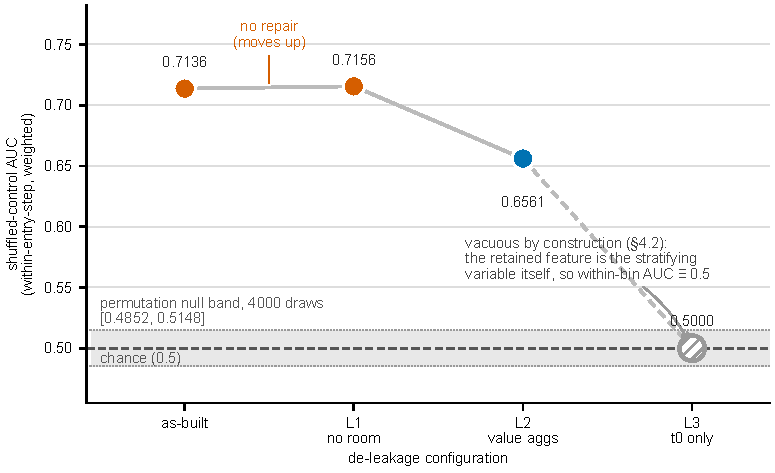
\includegraphics[width=0.50\textwidth]{figures/06_shuffled_trajectory.pdf}
\caption{The shuffled-control trajectory, trap versus post-de-leakage, on the
within-entry-step weighted AUC. The as-built configuration reads 0.7136;
dropping the calendar column alone reads 0.7156, \emph{above} it, so the path
moves the wrong way before it moves right. The strongest non-vacuous
configuration reaches 0.6561 and stops. The final point reads exactly 0.5000 and
is drawn hollow and hatched because it is fixed by construction, not
achieved.\label{fig4}}
\end{figure}

\section{Governance Implications, Conditional on the Bounds}

Every implication below is conditional on the bounds of \S4; none survives
transposition into an unconditional policy claim.

\begin{enumerate}\itemsep1pt
\item \textbf{Targeted dismantling is the only lever that moves the structure.}
Random removal needs about 60\% of the financial graph to halve its giant
component whereas degree-targeted removal needs 2.5\% (E6-fin). \emph{Condition:}
the giant component is a weak proxy at 47/49 saturated steps, so this is about
relative leverage, not absolute effect size.
\item \textbf{The illicit financial subgraph is a periphery, so act accordingly.}
Removing 100\% of illicit-labelled addresses leaves the component at 98.88\%
(E6-fin). \emph{Condition:} address-level enforcement is disruption of service
rather than damage to the network, and expecting network-level effects from it
is a category error our data bounds.
\item \textbf{The fast layer is where resilience lives.} 13.88\% of darkened
hosts return within a day at 6.2$\times$ chance (E7-inf) and median
infrastructure lifetime is 1.36 days (E0). \emph{Condition:} takedown cadence,
not takedown existence, is the operative variable at this layer.
\item \textbf{Domain infrastructure is the durable substrate.} Domain-hosted
infrastructure returns 1.31$\times$ as often as bare IP (80.77\% vs 61.49\%,
p \textless{} 0.001). \emph{Condition:} interventions that raise the cost of
domain re-registration attack the slower half of the churn cycle, and the feed's
scanner admixture is not separable.
\item \textbf{Displacement is directional: single-market seizures relocate rather
than remove.} Exposed vendors surface on Apollon at +10.5 pp above controls and
on Empire at +0.0, a zero-denominator cell that is unmeasurable rather than a
measured zero (E1-v3). \emph{Condition:} the corrected figures are two
non-significant point estimates, so the directional design and not the magnitude
is the finding, and +10.5 pp is an upper bound on substitution.
\end{enumerate}

\section{Limitations}

We consolidate, rather than disperse, the weaknesses a reviewer would find.

(i) \textbf{Causal magnitudes are not identified.} E3's design failed at matching
(overlap = 0.000), and with one ecosystem-wide shock no placebo or matching
machinery recovers an effect size; only H4 survives, and H4's support is the
confirmation of an absence, which is weaker evidence than a positive finding.
This is not a null result about the mechanism; it is the demonstration that this
data cannot support effect-size estimation in any design we could build.

(ii) \textbf{Historical windows.} The dated parts of the social and financial
layers cover roughly 2014--2017: the AlphaBay listings span 2014-12-21 to
2017-01-28, Agora 2014--2015, and the financial layer's ordinal axis maps to
approximately 2016-01-01 to 2017-11-03. Two social-layer panels (Kilos,
drug-listing) carry no date column at all, so no window can be stated for them,
and the current layer is infrastructure only.

(iii) \textbf{Censoring.} The social-layer outcome is first recorded feedback
rather than first transaction, and no seller key exists, so the event rate is a
lower bound and the standard errors are optimistic (E4). Both defects push every
duration estimate in the same direction, which is why the two medians are always
reported as a pair.

(vi) \textbf{Label provenance.} Elliptic++ labels are dataset-internal and
unverifiable against external ground truth, and the E5-fin gradient is equally
consistent with collection economics; the metrics that rest on this labelling
layer inherit this base.

Dropped limitations (metric-validity detail, external validation, novelty
exhaustiveness) are retained in Supplementary Notes S2 and S5.

\section{Conclusion}

We set out to measure the resilience of illicit data-trading ecosystems and
ended up measuring, just as much, the reliability of the measurement itself.
The protocol gates metrics before they are used, pairs every instrument with
controls that can actually reject, hash-manifests every reported number, and
keeps a public ledger of what failed. The controlled findings that survive are
modest in number and better attested than usual: churn-dominant infrastructure
with 6.2$\times$ reconstitution, a directional displacement whose magnitude is
bounded rather than estimated, and a structurally peripheral illicit financial
subgraph that can be removed in its entirety without moving the network's core.
They also rest on a thin dimensional base, since no resilience metric cleared
all three validity gates, and in a field where the resilience claims we build on
rest on measurements no control has tested, we accept that trade.


\bigskip
\section*{Supplementary information}
\noindent The Supplementary Materials contain the complete audit trail; every
number in the main text can be traced to a note below. Five notes are supplied
as a separate file (\texttt{supplementary.tex}).
\begin{itemize}\itemsep0pt
\small
\item \label{sup:S1}\textbf{Supplementary Note S1.} Complete protocol detail:
the two-list rule, the audit census, and the engineering discipline.
\item \label{sup:S2}\textbf{Supplementary Note S2.} The seven analyses' full
controls and rejected estimators, the specification-curve coefficients, the
exploratory cross-layer association, and the metric-validity matrix.
\item \label{sup:S3}\textbf{Supplementary Note S3.} Per-configuration anatomy
of the negative results (L1/L2/L3 de-leakage, the untrained floor, the
changepoint and infeasibility entries).
\item \label{sup:S4}\textbf{Supplementary Note S4.} Family-level
infrastructure profile, including the E0 survival panel (Supplementary
Fig.~S1), and the scenario-robustness analysis.
\item \label{sup:S5}\textbf{Supplementary Note S5.} Data, time coverage and
licence supplement, including the external-context source and the ethics
details.
\item \label{sup:A1A2}\textbf{Additional files 1 and 2.} The rule that draws the
census boundary, and the SHA-256 census of the 302 result artifacts, as two
plain-text files (\texttt{Additional file 1.txt}, \texttt{Additional file 2.txt}).
\end{itemize}

% Scientific Reports numbers references in order of first appearance, so the
% unsorted style is used.  (plainnat orders the list alphabetically by author,
% which would number the introduction's first citation far down the list.)
\bibliographystyle{unsrtnat}
\bibliography{refs}

\bigskip
\begingroup\small
\section*{Declarations}

\noindent\textbf{Availability of data and materials.} All source datasets are
public and are listed in Table~\ref{tab:data}. The analysis pipeline and the
audited result artifacts are openly available at
\url{https://github.com/chenyongjingg/illicit-data-economy-resilience}
(tag \texttt{v1.0}). The rule that fixes the census boundary of the result
manifest, and the SHA-256 manifest of all 302 result artifacts, are supplied
with this submission as two plain-text supplementary files (Additional file 1
and Additional file 2) and are carried in that repository as well;
Supplementary Note S1.3 summarises the census and Supplementary Note S5
records the licence detail.

\noindent\textbf{Competing interests.} The authors declare that they have no
competing interests, financial or non-financial. No author holds any interest
in, or has received any payment from, any organisation that would benefit from
or be harmed by the results reported in this manuscript.

\noindent\textbf{Funding.} This work was supported by the research project
``The Formation Mechanism of `Resilience' in the Illicit Data Economy and
Governance Countermeasures'', grant number 25CSH113, a public research grant
held by the authors' institution. The funder had no role in the study design, in
the collection, analysis or interpretation of data, in the writing of the
manuscript, or in the decision to publish.

\noindent\textbf{Acknowledgements.} Not applicable.

\noindent\textbf{Author contributions.} Z.X., Y.C. and S.Z. designed the study.
Z.X. and Y.C. assembled the data and ran the analyses. S.Z. supervised the
work. All authors wrote and approved the manuscript.

\noindent\textbf{Ethics statement.} The study uses only public metadata and
public archives; no leaked personal records were accessed; identifiers are
hashed; no interaction with illicit actors occurred. Two Gwern-curated sources
carry no explicit licence and are used under research fair use (Supplementary
Note S5). LLM-based tooling was used in exploratory analysis only, and no
reported number depends on LLM-generated labels. An early packaging artifact
contained a default service credential; it was rotated and purged from all
packaged snapshots.

\noindent\textbf{Additional file 1.} The rule that draws the census boundary
(which trees are walked, what counts as an artifact, and the per-tree counts that
sum to 302, so that the census count can be recomputed rather than taken on
trust). \emph{File format:} plain text. \emph{Supplied as}
\texttt{Additional file 1.txt}; summarised in Supplementary Note S1.3.

\noindent\textbf{Additional file 2.} The census itself: the SHA-256 digest of
each of the 302 result artifacts, one per line. \emph{File format:} plain text.
\emph{Supplied as} \texttt{Additional file 2.txt}.

\endgroup

\end{document}
